\begin{figure}[tb]
\centering
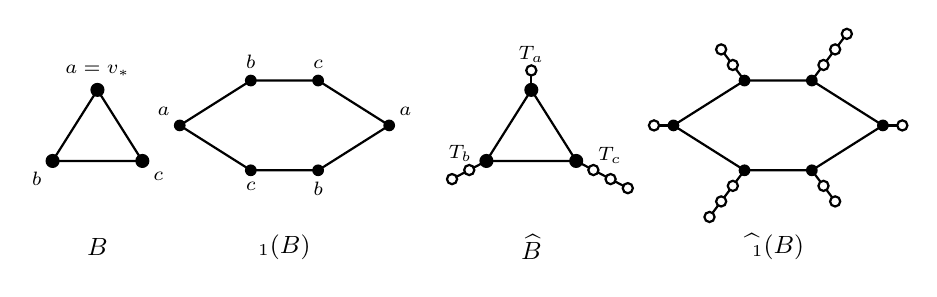
\begin{tikzpicture}[
  scale=.95,
  base/.style={circle,fill,inner sep=1.8pt},
  cfi/.style={circle,fill,inner sep=1.5pt},
  att/.style={circle,draw,fill=white,inner sep=1.3pt},
  lab/.style={font=\scriptsize,inner sep=1.5pt},
  line width=.8pt,
  every node/.style={font=\small},
]
\def\treeA#1#2{\draw (#1)--++(#2:.26) node[att]{};}
\def\treeB#1#2{\draw (#1)--++(#2:.26) node[att]{}--++(#2:.26) node[att]{};}
\def\treeC#1#2{\draw (#1)--++(#2:.26) node[att]{}--++(#2:.26) node[att]{}
                --++(#2:.26) node[att]{};}
\pgfmathsetmacro{\baseAngle}{atan2(.95/3,.6)}
\pgfmathsetmacro{\cfiAngle}{atan2(.6,.45)}
\foreach \attached in {0,1} {
  \begin{scope}[xshift={5.8*\attached cm}]
    \coordinate (a) at (0,.55);
    \coordinate (b) at (-.6,-.4);
    \coordinate (c) at (.6,-.4);
    \draw (a)--(b)--(c)--cycle;
    \ifnum\attached=0
      \node[base,label={[lab]above:$a=v_*$}] at (a) {};
      \node[base,label={[lab]below left:$b$}] at (b) {};
      \node[base,label={[lab]below right:$c$}] at (c) {};
      \node at (0,-1.55) {$B$};
    \else
      \treeA{a}{90}
      \treeB{b}{180+\baseAngle}
      \treeC{c}{360-\baseAngle}
      \node[lab,above] at (0,.85) {$T_a$};
      \node[lab,above] at (-.95,-.48) {$T_b$};
      \node[lab,above] at (1.05,-.5) {$T_c$};
      \foreach \v in {a,b,c} \node[base] at (\v) {};
      \node at (0,-1.55) {$\widehat B$};
    \fi
    \begin{scope}[xshift={(2.5+.8*\attached)*1cm}]
      \coordinate (a0) at (-1.4,.075);
      \coordinate (b0) at (-.45,.675);
      \coordinate (c0) at (.45,.675);
      \coordinate (a1) at (1.4,.075);
      \coordinate (b1) at (.45,-.525);
      \coordinate (c1) at (-.45,-.525);
      \draw (a0)--(b0)--(c0)--(a1)--(b1)--(c1)--cycle;
      \ifnum\attached=0
        \node[cfi,label={[lab]above left:$a$}] at (a0) {};
        \node[cfi,label={[lab]above:$b$}] at (b0) {};
        \node[cfi,label={[lab]above:$c$}] at (c0) {};
        \node[cfi,label={[lab]above right:$a$}] at (a1) {};
        \node[cfi,label={[lab]below:$b$}] at (b1) {};
        \node[cfi,label={[lab]below:$c$}] at (c1) {};
        \node at (0,-1.55) {$\CFI_1(B)$};
      \else
        \treeA{a0}{180} \treeA{a1}{0}
        \treeB{b0}{180-\cfiAngle} \treeB{b1}{360-\cfiAngle}
        \treeC{c0}{\cfiAngle}     \treeC{c1}{180+\cfiAngle}
        \foreach \v in {a0,b0,c0,a1,b1,c1} \node[cfi] at (\v) {};
        \node at (0,-1.55) {$\widehat{\CFI}_1(B)$};
      \fi
    \end{scope}
  \end{scope}
}
\end{tikzpicture}
\caption{A CFI-compatible rooted product for $B=K_3$ with $v_*=a$.
The hexagon labels indicate the base vertices of the fibres.
The attached paths $T_a,T_b,T_c$ have lengths one, two and three;
each vertex in the fibre over $z$ receives a copy of $T_z$.}
\label{fig:ss-cfi-example}
\end{figure}
